\documentclass[12pt, a4paper]{scrartcl}
\usepackage[utf8]{inputenc}
\usepackage{graphicx}
\usepackage{amsmath, amsthm, amssymb, textcomp}
\usepackage{setspace}
\usepackage{paralist}
\usepackage{graphicx}
\usepackage{caption}
\graphicspath{{WSK_im/}} %Graphic is in a folder named WSK_im in the currend directory
\usepackage{float}
\usepackage{authblk}
\renewcommand\Authfont{\fontsize{12}{14.4}\selectfont}
\title{Bayesian probability theory - Lesson 9}

\author{Wolfgang von der Linden}
\date{Transscript}

\begin{document}
\setlength{\parindent}{0pt}
\maketitle
\onehalfspacing
Welcome to unit 9, the last unit of this course on Bayesian probability
theory. My name is Wolfgang von der Linden and I will enable you to
help Captain Bayes and her crew to get familiar with  \textbf{Bayesian simulation
techniques}.
This unit is dedicated to  \textbf{Monte Carlo methods} and  \textit{efficient stochastic algorithms}.\\
\begin{itemize}
\item We will learn how stochastic algorithms can be used to \textit{compute quantities of interest}, like the number of $\pi$,
\item we will learn how to \textit{quantify the uncertainty} and to \textit{derive the probability distribution} for the desired quantity
\item and we will learn clever Monte Carlo techniques including  \textbf{Nested Sampling}.
\end{itemize}

\section*{Finding $\mathbf{\pi}$}
In the adventure Captain Bayes proposed to determine $\pi$ - the ratio of the circumference of a circle to its diameter - by a random experiment. 
You just need a stick of a certain length l
and some straight parallel lines which have a distance d each. Then, you just throw the stick repeatedly on the array of lines and you count how
often it cuts a line. You can estimate $\pi$ from the ratio $\frac KN$ given by the number of cuts K
divided by the number of throws N.\[\pi\approx 2\frac KN\frac ld\]

Let’s see how we can justify this relation that Captain Bayes had in mind.
To keep the discussion simple, we assume from now on that the \textit{length of the
sticks is equal to the distance between the lines}.
By $a$ we denote the distance of the midpoint of the stick to the nearest line.
The angle between the stick and the lines is denoted by $\phi$. This is enough
information to decide whether a stick cuts a line or not: 
The stick cuts the nearest line if its extension from the midpoint to the tip
perpendicular to the line exceeds the distance $a$.\\%9_1
 \begin{figure}[H]
	\centering
	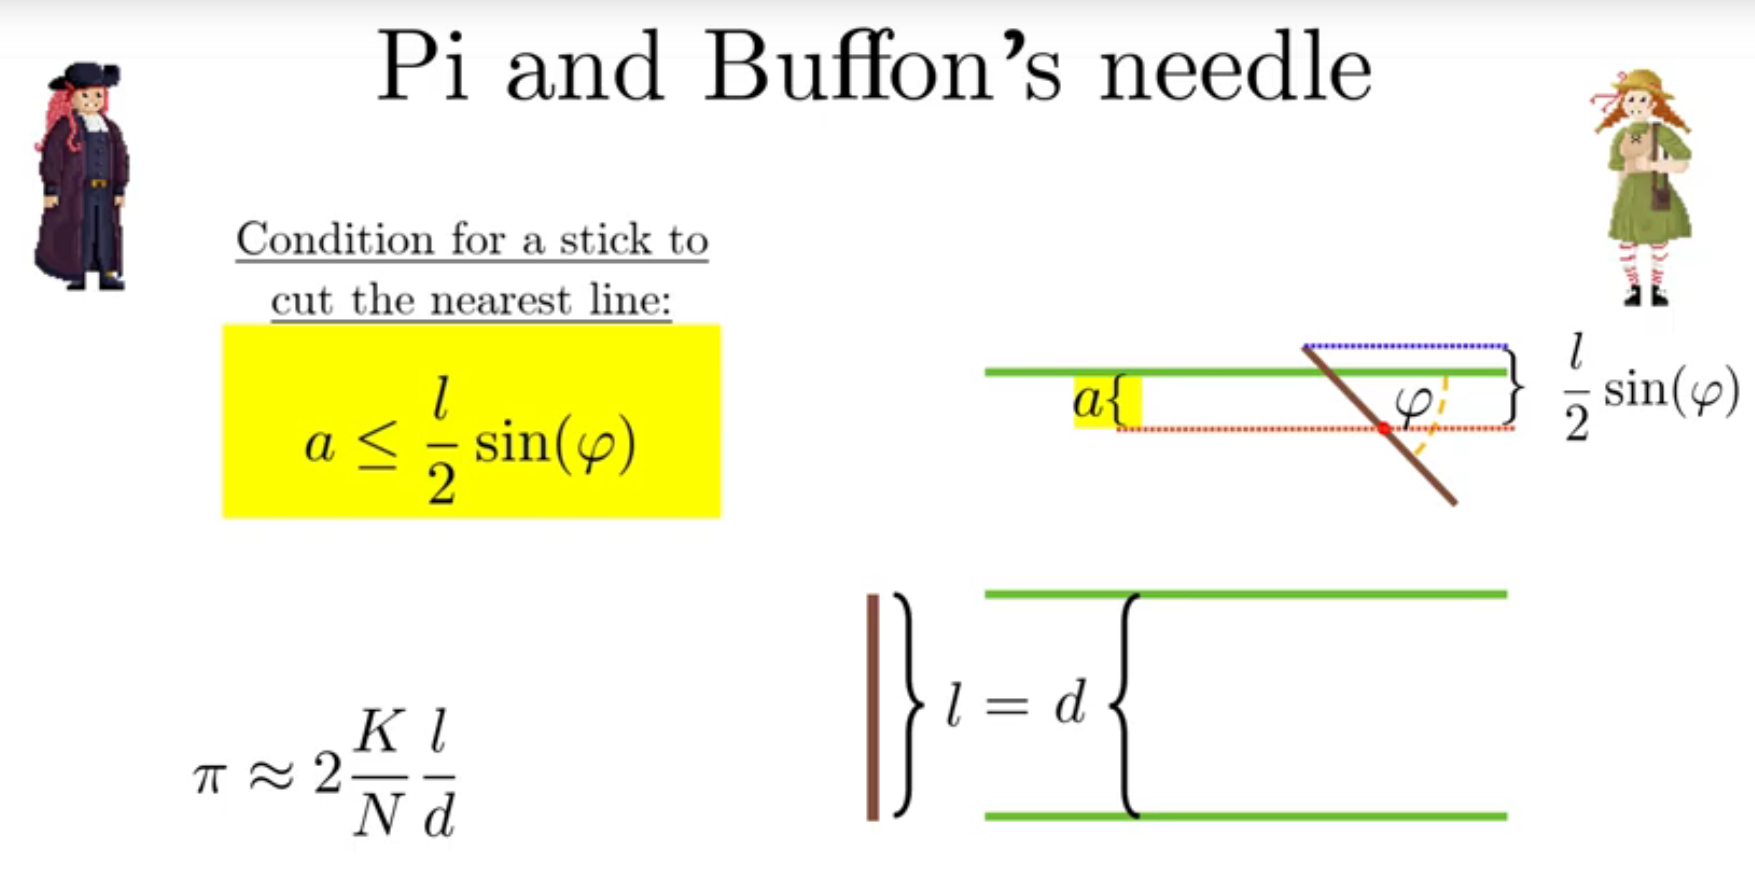
\includegraphics[width=0.75\textwidth]{9_1.png}
\end{figure}

Let’s visualize the possible and favorable stick orientations in the following
$a$-$\phi$ plane:\\
1) phi ranges from zero to $\frac{\pi}{2}$ and the parameter a is between 0 and
L/2. Therefore the area of possible events is given by the product of
the ranges.\\%
2) The favorable orientations of the stick - so the ones where it intersects a line - are
given by the area under the curve $L/2sin(\phi)$.%

That results in the area of favourable events of L/2.\\%9_2
 \begin{figure}[H]
	\centering
	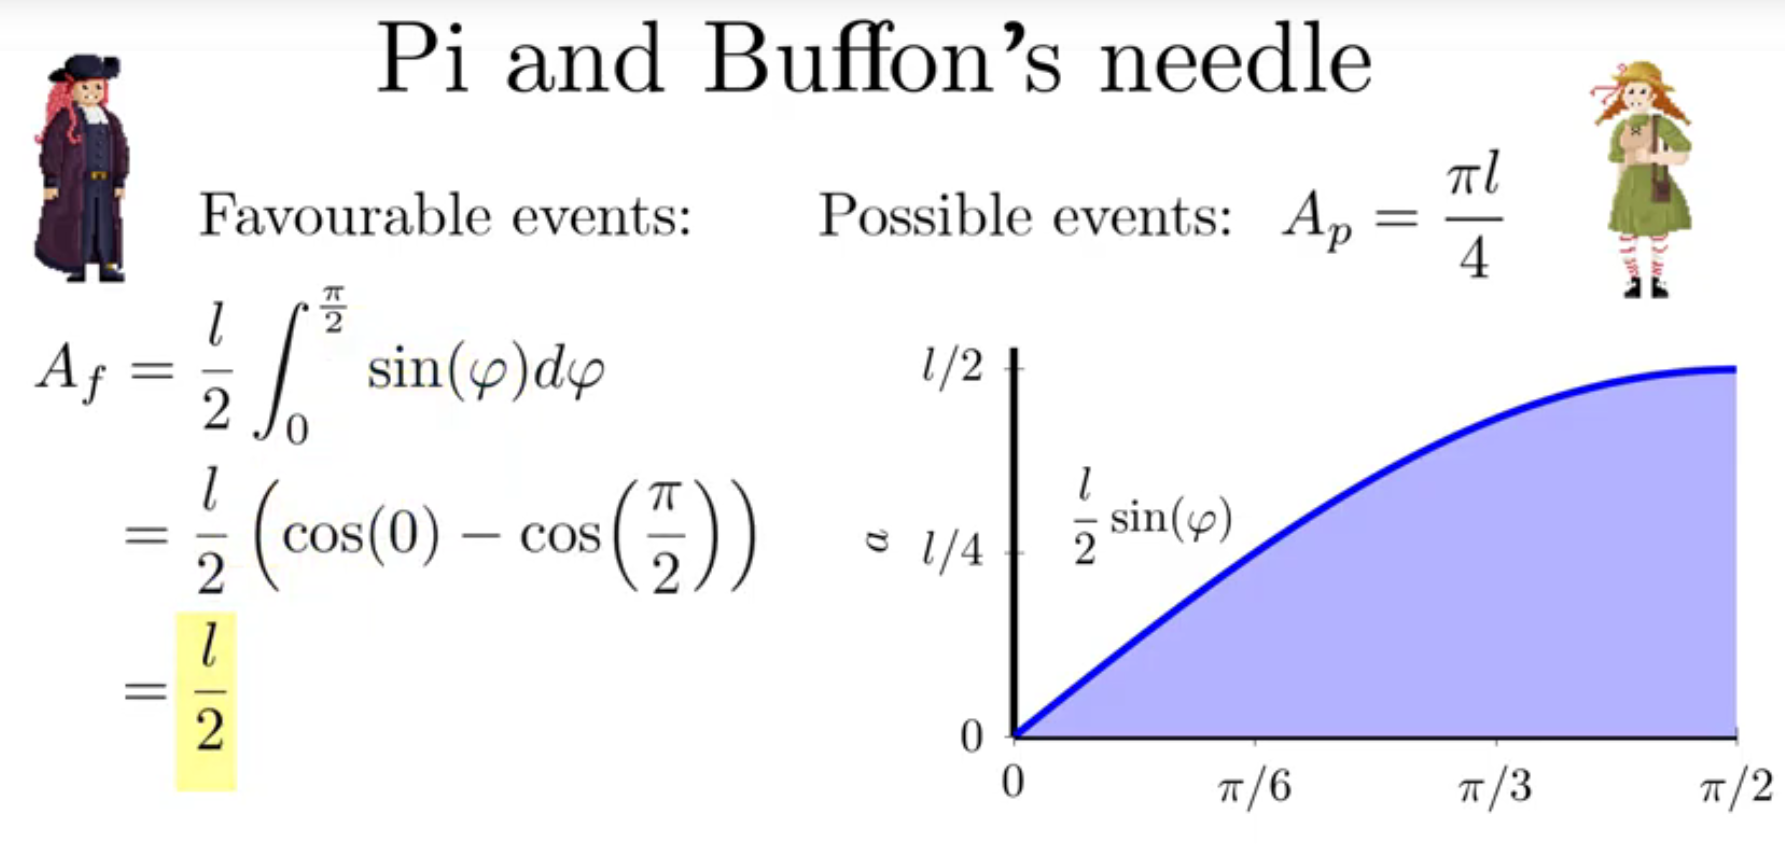
\includegraphics[width=0.75\textwidth]{9_2.png}
\end{figure}

Thus, the probability that a randomly thrown stick cuts one of the parallel
lines is given by the ratio of the areas, resulting in $\frac{A_f}{A_p}=\frac{2}{\pi}$.\\%

In the limit of infinite throws, the  \textbf{law of large numbers} tells us that the ratio K/N approaches the intrinsic probability.
That implies that $2N/K \rightarrow \pi$.

A finite number of throws 2N/K then corresponds to the approximation proposed by Captain Bayes. A warning is in order here: We know that
K/N is an \textit{unbiased estimator} for the intrinsic probability q. The inverse
N/K, however, is  \textbf{not} an unbiased estimator for 1/q because \textit{the mean of 1/X is not the same as 1 over the mean of X.}
\begin{equation*}\boxed{\left\langle \frac 1x \right\rangle \neq \frac{1}{\langle x\rangle}
}\end{equation*}\\

The warning becomes even more urgent if looking at \textit{transformations
of errors}. Assume you have a measure $\Delta q$ for the error of q for instance the standard
error, then the error of 1/q
\textbf{won’t} be $1/\Delta q$.
\textit{As a side note, it is worth mentioning that the propagation of experimental errors can also be treated with the rules of probability theory.}\\

\fbox{\parbox{\linewidth}{\textbf{Question 1.} You measured a quantity x=3cm with an error of $\Delta$x=0.1cm. \\
You are insterested in the error $\Delta$y of the value y given by the relation y= $\frac{2}{x^2}$.\\
Which of the following statements are correct?\\
a) The error can be obtained by Taylor expansion and reads $\Delta y = |y'(x)|\Delta x$\\
b) The relative error is approximately $\frac{\Delta y}{y}=\frac{1}{15}$\\
c) The relative error is approximately $\frac{\Delta y}{y}=\frac{1}{30}$\\
d) The error is $\Delta y =\frac{3}{\Delta x^2}$
}}
\\

Although Captain Venn, who just arrived, would be satisfied with this
asymptotic limit, Captain Bayes would like to answer Lyra’s question about
\textit{how long it takes to get a reliable result for the first four digits}. Captain
Venn could argue that he knows the variance of the 2N/K estimator for
$\pi$, based on the law of large numbers. However, the latter applies to the
inverse K/N and not directly to N/K. \\

One can do a Taylor expansion%9_3
 \begin{figure}[H]
	\centering
	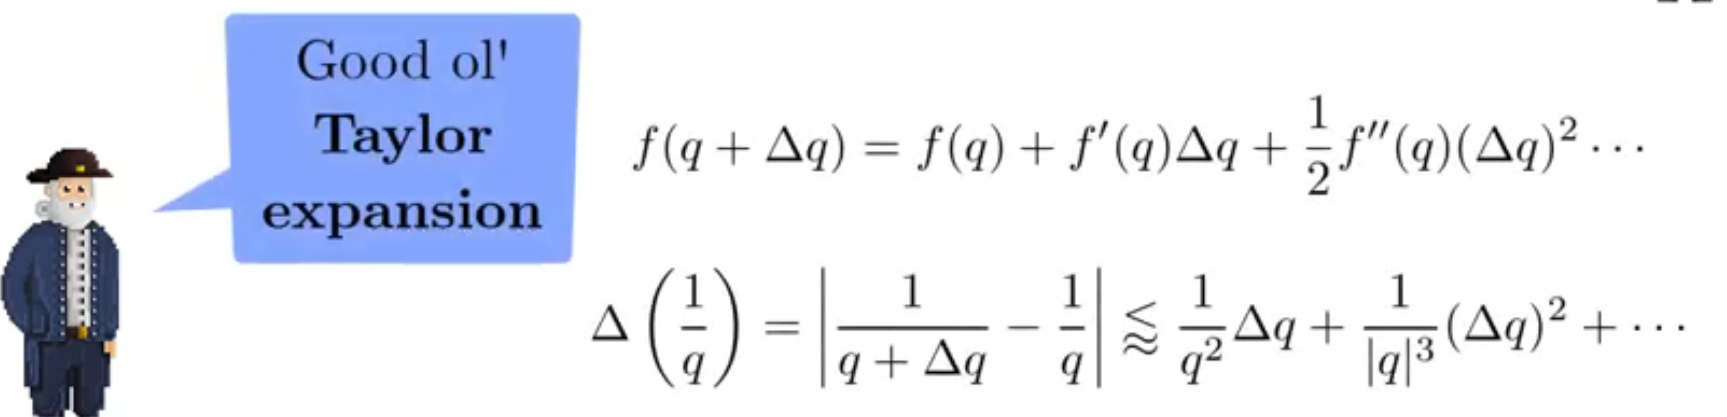
\includegraphics[width=0.75\textwidth]{9_3.png}
\end{figure}
 to
overcome this problem for very large values of N, but for general N and
for a systematic approach, the Bayesian way is to \textit{determine the posterior
probability density $p(\xi|K,N)$ for the numerical value $\xi(\pi)$} based on a
finite number of throws N and the observed number of intersected lines.
From the posterior density she would then compute the
moments in the usual way.
\[\langle \xi^k\rangle = \int \xi^kp(\xi|K,N)d\xi\]
For the posterior we invoke Bayes’ theorem to obtain the product of likelihood
and prior.
\[p(\xi|K,N)=\frac 1Z p(K|\xi,N)p(\xi)\]
The moments can then be calculated as integral over likelihood times prior
with the explicit normalization.
\[Z=\int p(K|\xi,N)p(\xi)d\xi\]
Now it is advantageous to introduce a variable transformation from $\xi$ to the
cut probability q, because then likelihood and prior are
easier to grasp:
\[\xi=\frac 2q\]
The likelihood then turns into  the  \textbf{binomial distribution}
\[p(K|\xi,N)\rightarrow p(K|q,N)={N\choose K} q^K(1-q)^{N-K}\]
and for the prior p(q) we assume for simplicity the  \textbf{uniform distribution} on
the unit interval. \[p(\xi)\rightarrow p(q)=1 \quad q\in[0,1]\]
The remaining integrals involve  \textbf{Beta-functions} and can be
determined analytically. \footnote{Have a look at the bonus material!} The final result for the mean is almost identical to
the approximation Captain Bayes proposed 
\begin{equation*}\boxed{\langle \xi\rangle = 2\frac{N+1}{K}
}\end{equation*}\\
and it converges towards $\pi$ for $N\rightarrow \infty$, for the same reason outlined before.\\

Finally, to answer the question of Lyra we consider the the \textbf{variance}. 
As we want to know \textit{how many steps} it takes to reach a four-digits accuracy,
we can assume that both N and K are much greater than 1. Then the
variance and its square root, the uncertainty, simplify further
and we obtain the ubiquitous $\frac{1}{\sqrt{N}}$ dependence with a
pre-factor that is roughly 4.%9_4
 \begin{figure}[H]
	\centering
	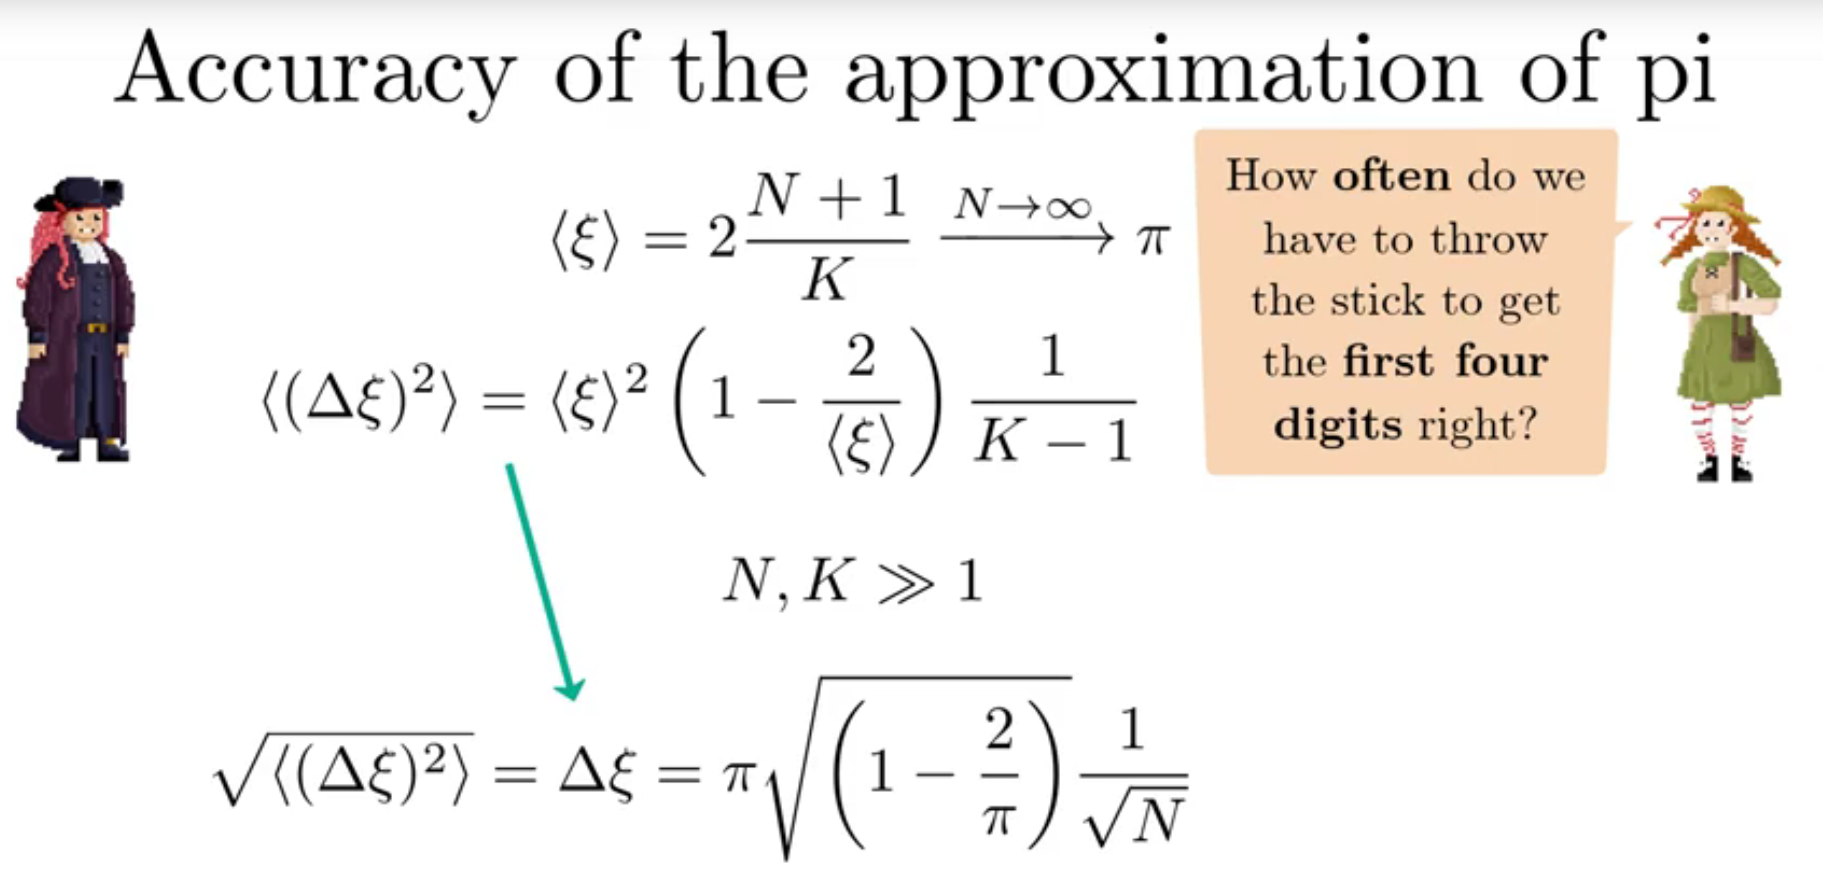
\includegraphics[width=0.75\textwidth]{9_4.png}
\end{figure}
In order to have m fractional digits accuracy, $\Delta \xi$ has to be less than $10^{-m}$, we obtain \[\frac{\pi^2(1-\frac{2}{\pi})}{N}\leq 10^{-2m}\]

Lyra, was eager to see how long it takes to get the first four digits right,
which corresponds to 3 fractional digits. The answer for
Lyra is: It takes 6 million throws.\\

\fbox{\parbox{\linewidth}{\textbf{Question 2.} Which of the following statements regarding the derived accuracy are correct?\\
a) To have a certainty of approx. 95\%, one should throw 8 million sticks.\\
b) The probability to have 4 digits right when throwing the stick approximately 4 million times is roughly 67\%.\\
c) After 4 million throws, the first four digits are correct.
}}
\\

\section*{Multidimensional integrals}
In the previous example the integral over the posterior was one-dimensional
and it could be evaluated analytically. Unfortunately, this is rather the exception and not the rule.
Say we are interested in the \textit{density profile within a cross section of a
fusion plasma}. Since the temperature of a plasma is typically around 100 million
Kelvin, you can’t put measuring devices inside the plasma, they would
just melt away. But the plasma emits X-rays and their  \textbf{emissivity} can be
measured by cameras outside the plasma. The emissivity is \textit{proportional to
the integral over the density} along the line along which the camera looks
into the plasma.
\[I_{\nu}\propto \int_{L_{\nu}}\rho(\vec{x})ds\]
Say we are interested in the density in a 2D cross section at 100 × 100 points
and we want to determine it without resorting to a parameterised model.
This so-called  \textbf{form-free reconstruction} then has 10000 unknown parameters.\\

The problem is related to the  \textbf{Abel-transform}, if the plasma density is axial
symmetric and noise-free. 
\begin{equation*}\boxed{F(y)=2\int_y^{\infty}\frac{f(r)r}{\sqrt{r^2-y^2}}dr
}\end{equation*}\\
Here, both conditions are not met and typically,
there are much less line-integrals than unknowns. So we have an \textit{under determined ill-posed inversion problem}. It could not be worse.
Nevertheless, Bayes’ theorem allows to infer the density vector $\vec{\rho}$, corresponding to the values on the grid.
\[p(\vec{\rho}|d)=\frac 1Z p(d|\vec{\rho})p(\vec{\rho})\]
Z is, as always, the normalization. Here, as with all underdetermined problems, the prior plays an important role and a generalized \textbf{entropic prior} is well suited, one that takes into account, that the testable information, provided by the data, is corrupted by noise. This approach is called:  \textbf{Quantified Maximum Entropy}\\

\fbox{\parbox{\linewidth}{\textbf{Question 3.} What is an entropic prior?\\
a) A prior that is derived by using the maximum entropy principle.\\
b) A prior that considers some constraints but otherwise is maximally uninformed.\\
c) A prior that is scale-invariant and guarantees a normalization of one.
}}
\\

This example should only show you a real-world example, in which a high-dimensional integral occurs. We do not want to go into detail of the posterior
here, but rather demonstrate how we can compute mean values of some
observables f($\vec{\rho}$) like  \textbf{mean density} and  \textbf{covariance}. To this end you have to
evaluate 10000-dimensional integrals of the following form.
\[I=\langle f(\vec{\rho})\rangle = \int dV_{\vec{\rho}}f(\vec{\rho})\frac{w(\vec{\rho})}{Z}\]

If we would use standard quadrature methods, with say 10 integration points
per dimension, we would have to evaluate the posterior $10^{10000}$
times. If each evaluation could be done on an atomic times scale, say in
Femto seconds, it would still take $10^{9977}$ years. The Big bang happened
roughly $10^{10}$ years ago. So it would take $10^{9967}$ big bangs before the computer spits out the result; not to mention how it can survive it all. This impressively
illustrates the  \textbf{curse of dimensionality}.\\

\section*{MCMC - Markov Chain Monte Carlo}
Fortunately, we can overcome it by using probabilistic ideas. We have learned
in previous lessons that we can \textit{estimate the mean} of a function f($\vec{\rho}$) based on independent samples drawn from the posterior
and we also know how to \textit{estimate the variance}
to have a measure for the uncertainty for the estimate of the mean.\\%9_5
 \begin{figure}[H]
	\centering
	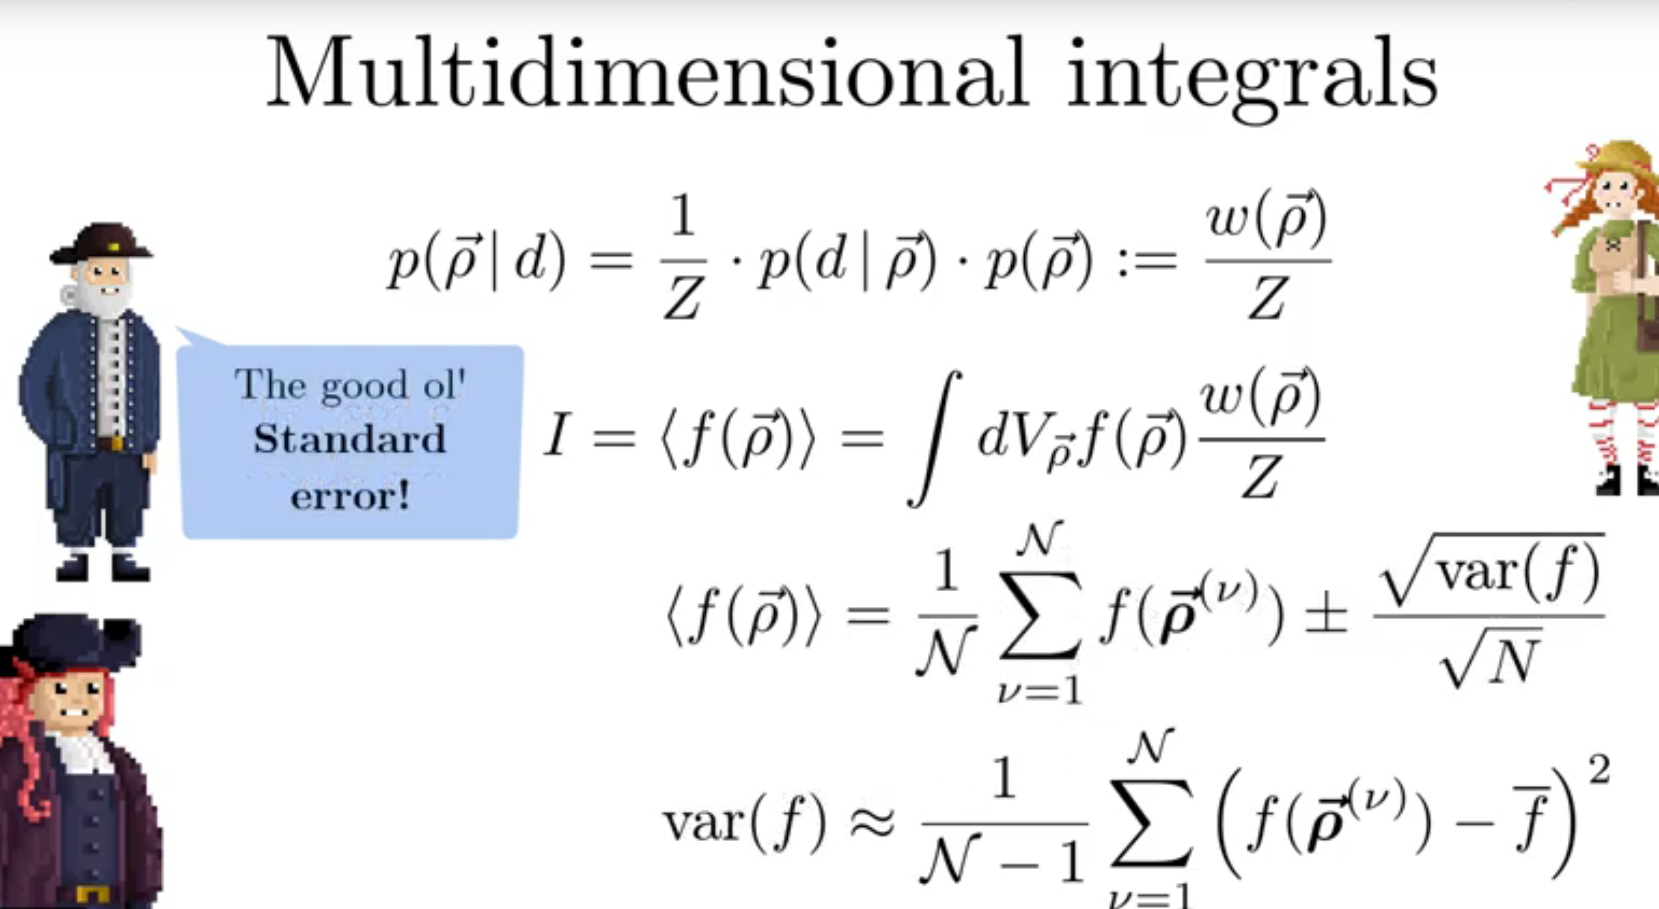
\includegraphics[width=0.75\textwidth]{9_5.png}
\end{figure}

The crucial aspect is that in many cases the uncertainty is more or less
\textit{independent of the dimension} and the uncertainty can be reduced by $\sqrt{N}$ (see formula in picture above) term to reach fairly reliable results. 
So we see that
the curse of dimensionality disappeared and that the problem boils down to
generating independent samples from the posterior.\\

\fbox{\parbox{\linewidth}{\textbf{Question 4.} Which statements are correct regarding the curse of dimensionality?\\
a) The curse of dimensionality can be overcome by using samples and reformulating the problem as a one-dimensional one.\\
b) The curse of dimensionality can be overcome by using random samples that fill the full sample space uniformly. An integral can be approximated by evaluating quadrature formulas at randomly sampled pivot points.\\
c) The computational effort to evaluate integrals numerically scales exponentionally with the number of dimensions d.
}}
\\

The task of generating independent samples from a pdf was already
solved in the Manhattan Project some 80 years ago. The idea is pretty
simple, but the proof is a bit tricky. Here is the recipe:\\

We start with a randomly selected initial density profile. Let’s skip
some initial iterations and assume n elements of the sample have already
been created. 
Starting from the current density, the next element is generated by the
following steps:
\begin{enumerate}
\item Make a small change to the current density and call it a \textbf{trial}. 
This can be done, for instance, by adding a Gaussian random number
to one of the components of the density vector.
\item Compute the ratio of the posterior for the trial and the current
density and compute from that the so-called  \textbf{acceptance probability $P_a$}
\item The trial density is accepted with that probability by drawing
a uniform random number r from the unit interval, and \textit{if r is less than
the acceptance probability} the trial density is accepted, otherwise it is
rejected.
\item The next element of the sample is the trial density, if it is
accepted, otherwise it is again the current density.
\end{enumerate}%9_6
 \begin{figure}[H]
	\centering
	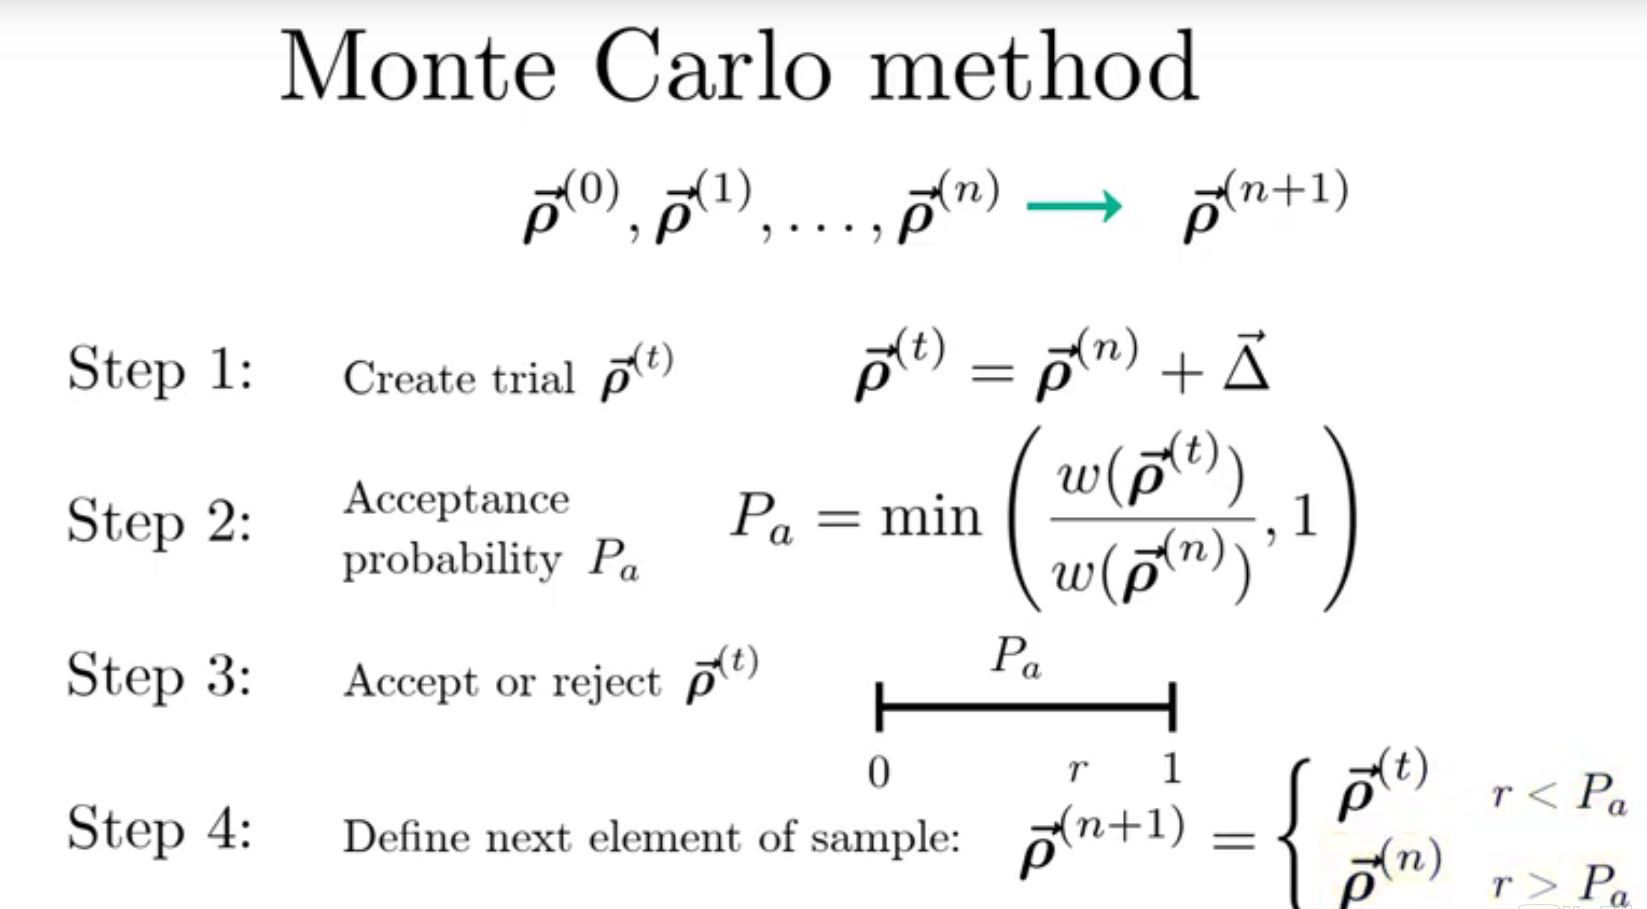
\includegraphics[width=0.75\textwidth]{9_6.png}
\end{figure}

\fbox{\parbox{\linewidth}{\textbf{Question 5.} How is this stochastic process called?\\
a) Gaussian process\\
b) Random walk\\
c) Markov process\\
d) Wiener process
}}
\\

Right, it’s a  \textbf{Markov process} and that is why the approach is called  \textbf{MCMC:
Markov Chain Monte Carlo}. But more precisely, we are using the  \textbf{Metropolis
algorithm} for the individual steps. \\

\fbox{\parbox{\linewidth}{\textbf{Question 6.} What is the Markov Chain Monte Carlo algorithm good for?\\
a) To evaluate mean values of a probability distribution.\\
b) To evaluate the normalization of a probability distribution.\\
c) To generate or draw a sample according to a given probability distribution.\\
d) To find the maximum of a probability distribution.
}}
\\

\section*{Nested Sampling}
We have seen that for the evaluation of mean values we do not need the
normalization of the posterior, as it drops out in the acceptence probability. For that reason these MCMC algorithms cannot be used to compute the normalization.
But for many problems it is of central importance, for instance for \textit{model comparison}
as outlined earlier. So we need a different tool to \textit{compute high dimensional
integrals over likelihood times prior}.
\[Z=\int L(\Vec{x})p(\vec{x})dV_{\vec{x}}\]

A similar expression is at the heart of statistical physics, the  \textbf{partition function}:
\[Z=\int_{\Omega} e^{-\beta H(x)}dx\]
Once we know the partition function we can determine all other thermodynamic
variables. A particularly challenging situation is encountered in physical systems at first order phase transitions.

There are a few methods that allow the numerical computation of such integrals but the most promising one has been found in the treasure box by Captain Venn:  \textbf{nested sampling}. That is an approach that recently has been proposed by John Skilling.
Nested sampling makes use of  \textbf{Lebesgue integrals} by \textit{transforming the high-dimensional integral} over the space spanned by the vectors $\vec{x}$ into a one-dimensional integral over the possible values of the integrand:
\begin{equation*}\boxed{\int f(\vec{x}p(\vec{x})dV_{\Vec{x}} \rightarrow \int X(f)df \qquad X(f)=\int_{f(\vec{x})>f}p(\vec{x})dV_{\vec{x}}
}\end{equation*}\\

Here X(f) is the integral over the prior enclosed by the contour given by f(x) = f.
This object X(f) is therefore the  \textbf{restricted prior mass}. Let’s consider a very simple
example with a prior p(x) = x restricted to the interval [0, 2] and a function $f(x) = x^2$ that ranges from [0,4]
Then the integral of interest yields 4.
\[Z=\int_0^2x^2xdx=4\]

Then the constraint according to the contour results in the restricted prior mass
\[X(f)=\int_{x>\sqrt{f}}^2p(x)dx=l-\frac f2 \Rightarrow Z=\int_0^4\left(2-\frac f2 \right)df=4\]
From that, the Lebesgue integral also yields the value 4.\\

\fbox{\parbox{\linewidth}{\textbf{Question 7.} Another example for you as exercise:\\
Given is a pdf on the unit circle $p(x,y)=\frac{2}{\pi}(x^2+y^2)$.\\
1) Proof that this pdf is normalized on the unit circle (i.e. for $|\vec{x}|\leq 1$).\\

2) The function (e.g. the Likelihood) is defined as follows:\\
$f(x,y)=x^2+y^2$\\
What is the range of f?\\

3) Calculate $X(f)=\int_{f(\vec{x})>f}p(\vec{x})d\vec{x}$.\\

4) Proof that $\int_{|\vec{x}|<1}f(\vec{x})p(\vec{x})d\vec{x} = \int_fX(f)df=\frac 23$
}}
\\

As outlined in the attached notes of John Skilling\footnote{see bonus material} the plausibility argument
for Nested Sampling is the following:\\
 Draw an ensemble of \textit{n random locations
x} according to the prior pdf, each of which has its own value f(x), which we
can \textit{place in ascending order}. Crudely, if we discarded the lower half of the
values, the survivors would be \textit{random samples} from the prior, taken within
the \textbf{restricted volume} corresponding to $f(x) > f_{median}$. And, statistically,
that restricted volume would be roughly half the original volume because
that’s what a median is.%9_7
 \begin{figure}[H]
	\centering
	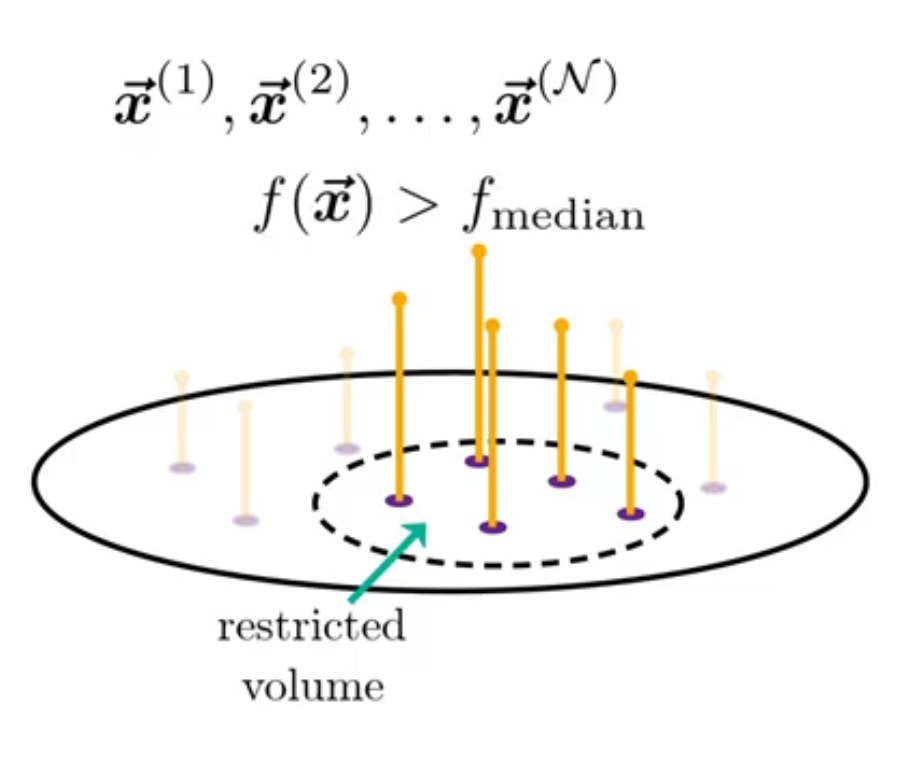
\includegraphics[width=0.6\textwidth]{9_7.png}
\end{figure}
By ordering the samples according to their f-value, we can \textit{infer on the prior masses}. Repeating that procedure r times would yield  \textbf{compression of the prior mass X(f)} by a factor something like $2^{-r}$. 
\[X(f_{median}^{(r)})\lessapprox 2^{-r}X(f_{median}^{(0)})\]
This is the exponential behaviour required to overcome the curse of dimensionality.\\

So how does Nested Sampling actually work?
As mentioned, we rewrite the high dimensional integral into a one-dimensional integral.
Now the next logical step is a  \textbf{discretization in f}.\\%
\begin{equation*}\boxed{Z\approx\sum_nX(f_n)(f_n-f_{n-1})=\sum_nf_n(X(f_n)-X(f_{n+1}))
}\end{equation*}\\
The only (but decisive) problem is that \textit{we don’t know the constraint prior mass
X(f)}. John Skilling introduced an ingenious algorithm of choosing $f_n$ sta-
tistically in the following sense, which is slight modified as compared to the
scheme mentioned at the beginning:
\begin{enumerate}
\item initialize a counter n = 1
\item set the first value $f_n$ to the lower bound of the function f(x): $f_1=min(f(x))$
\item generate a sample $\{\vec{x}\}_{\nu=1}^N$ of size N according to the prior with a
constraint $f(\vec{x}_{\nu}) > f_n$
\item compute the corresponding f-values $f_{\nu}=f(\vec{x}_{\nu})$ and determine the smallest
one and call it $f^*=min(f_{\nu})$
\item increment the counter n and set $f_n=f^*$

\item Now repeat the steps 3-5 until suitable convergence is achieved.
The estimation of the integral now uses the sequence of f-values generated in
this way.
\[Z\approx\sum_{n=1}^{N_{max}}f_n(X_{n+1}-X_n)\]
\end{enumerate}
We still don’t know the X-values $X_n$ corresponding to the f-values, but
now we can determine them statistically.\\

The explanation in a nutshell goes as follows: The X-values $X_n$ corresponding to the sequence of f-values $X_n=X(f_n)$ are uniformly distributed. The smallest
f-value of the sample corresponds to the largest X-value, because by construction, X(f) is a \textit{monotonically decreasing function in f}. Then we can use
 \textbf{order-statistics} to determine the pdf $p(X_n)$ From that, we can generate a
sample of X-values $X_n$ that corresponds to the sequence of f-values.\\

Nested sampling can even be used to solve really tough physical problems.
For instance, it allows to determine the  \textbf{critical exponents} and many other observables
of the  \textbf{Potts model} that exhibits a phase transition of second or first order
depending on a parameter of the model.\\


This concludes Unit 9 and we have reached the end of the entire course. In
this unit, we learned how stochastic simulation techniques work and how
Bayesian probability theory helps to estimate errors.\\
We have seen how Markov Chain Monte Carlo methods can be used to tame
high dimensional integrals to calculate the desired moments of a probability distribution and also how to evaluate partition functions and evaluate
normalization terms using the recently proposed Nested Sampling technique.\\

Have a look at the bonus material and the interactive Pluto notebooks to get
deeper insights into these technics and explore the vast configuration space
of Sudoku.
Please feel free to ask questions in the forum and feel encouraged to test your
knowledge in the quiz!
We hope you enjoyed this course and our adventures with Captain Bayes
and her crew. You are now equipped to apply Bayesian probability theory in
your daily applications, you have learned the skills to update your knowledge
base and you should feel better prepared to face uncertainty! :-)
%bayes pic 9_8
 \begin{figure}[H]
	\centering
	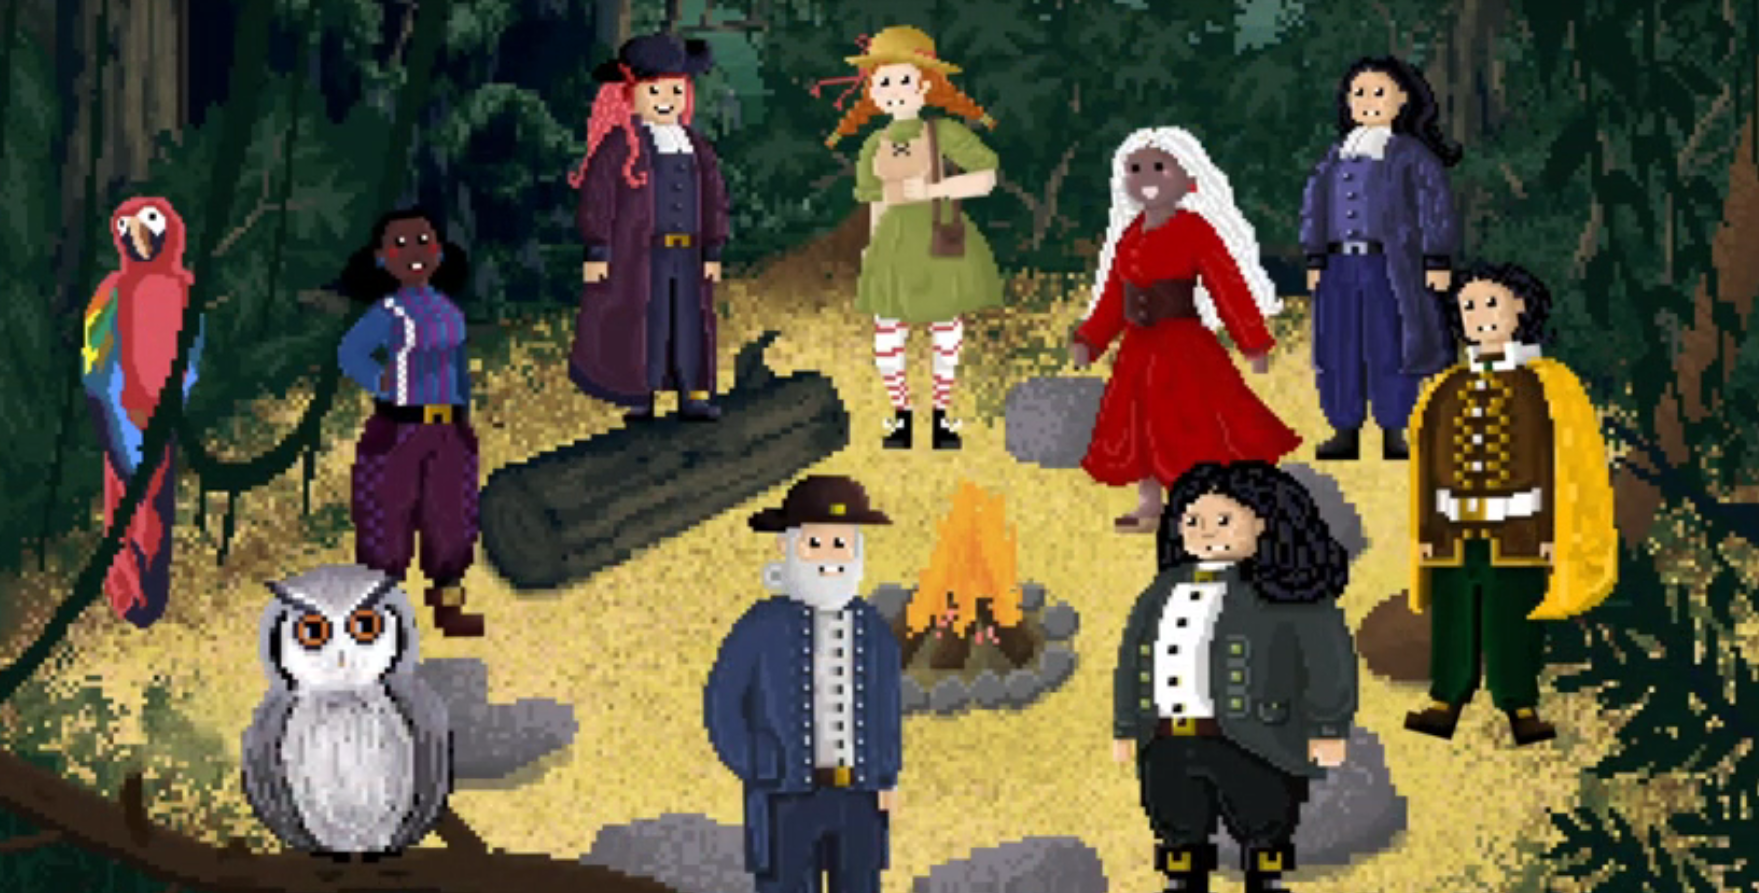
\includegraphics[width=0.6\textwidth]{9_8.png}
\end{figure}

\end{document}